\documentclass[11pt,a4paper]{article}
\usepackage{amsmath,amsfonts,amsthm,amssymb}
\usepackage[colorlinks,linkcolor=blue,urlcolor=blue]{hyperref}
\usepackage{graphicx,float,wrapfig,subfig}
\usepackage{xeCJK}
\usepackage{fontspec}
\usepackage{enumerate}
\usepackage{setspace}
\usepackage{indentfirst}

% Chinese support
\setCJKmainfont[BoldFont={Adobe Heiti Std}, ItalicFont={Adobe Kaiti Std}]{Adobe Song Std}
%\setCJKsansfont{WenQuanYi Zen Hei}
\setCJKmonofont{Adobe Fangsong Std}
\punctstyle{quanjiao}

% Spacing and margins
\onehalfspacing
\allowdisplaybreaks
\parindent=2em
\parskip=1ex
\addtolength{\hoffset}{-2em}
\addtolength{\voffset}{-10ex}
\addtolength{\textwidth}{4em}
\addtolength{\textheight}{5ex}


\begin{document}

% Make title
\title{\textbf{第16届智能体大赛规则}}
\author{\texttt{清华大学计算机系科协}}
\date{\today}
\maketitle
\thispagestyle{empty}

% Homework begin from here
\section{概况}
本届智能体大赛游戏名称为``战火星空'',采用了经典的飞行射击游戏做为游戏背景。

选手双方分别作为Boss和Plane,在规定的时间内,Boss发射子弹,Plane躲避子弹并尽可能地停住攻击Boss,以此获得积分。此外,Plane还有额外的技能可以使用。

两位选手交换角色进行2场比赛,比较各自Plane的得分即可决出胜者。

以下,我们将对游戏的规则做更为具体的介绍。

\section{游戏运行机制}
本游戏是即时策略游戏,但可以认为是时间间隔比较小的回合制游戏。每0.1s作为一个回合,游戏最多进行3000回合,即5分钟。在此期间,玩家双方需要不断根据当前的游戏局面做出相应的指令。

游戏结束条件有以下2种:
\begin{enumerate}[(a)]
\item Plane被Boss发射的子弹击中。
\item 3000回合到。
\end{enumerate}

\subsection{Boss的机制}
Boss是固定与屏幕上方的一个战舰,可以从一个固定点发射匀速飞行的圆形子弹。

一共有5种不同类型的子弹,它们的速度、半径以及受到的限制各不相同。对某类子弹的限制体现为,在任意时刻,屏幕上该类子弹的数目不能超过一个给定的值,\textbf{并且,每回合发射该类子弹不超过max(0.4 * 剩余可发子弹数, 6)个}。

玩家需要根据游戏局面信息,控制Boss发射新子弹,指定其速度和发射时间。

\subsection{Plane的机制}
Plane是一个可以在屏幕上移动的小飞机,它在静止时会默认向Boss发射子弹,每静止一个回合即发射一枚子弹。

Plane的移动速度有一个上限,在正常状况下不能超过该上限。

\textbf{Plane每存活100回合,会获得一个技能点}。

Plane具有两个特殊的技能:
\begin{enumerate}[(a)]
\item 加速\\
使用该技能会让Plane的速度上限变为原来的2倍,持续3秒钟。\textbf{损失2个技能点}。
\item 清屏\\
使用该技能会瞬间清楚屏幕上的所有子弹。\textbf{损失5个技能点}。
\end{enumerate}

\subsection{胜负判定}
游戏采取积分制,积分即Plane打中Boss的次数,等价于Plane静止的回合数。

两位选手进行PK的规则是,玩家1先作为Boss,玩家2先作为Plane,二者进行比赛,记录得分。接下来,两玩家交换角色再进行一场比赛,记录得分并与之前的得分比较,分数高的一方获胜。

\section{游戏参数}

\texttt{游戏参数可能会随着比赛的进行做一些小范围的修改以保证游戏的平衡性与可玩性,请时常关注比赛网站\url{http://ai.net9.org}以获得最新的规则信息。}

\subsection{游戏屏幕坐标和尺寸}
如图~\ref{fig:coor}所示。
\begin{figure}
\centering
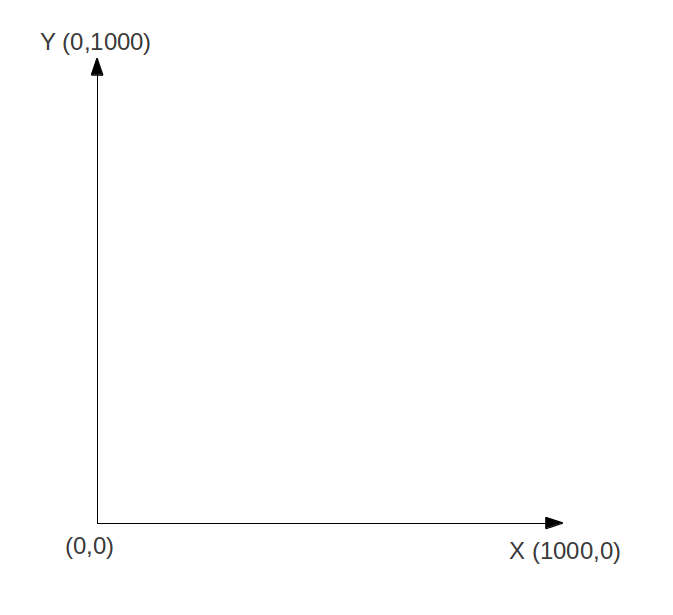
\includegraphics[width=0.4\textwidth]{coor.png}
\caption{游戏屏幕坐标和尺寸}
\label{fig:coor}
\end{figure}
\subsection{Boss发子弹的限制}
\begin{enumerate}[(a)]
\item 子弹发射点固定为$(500,800)$。
\item 子弹参数
\begin{center}
\begin{tabular}{|c|c|c|c|c|c|}
\hline
子弹类型&1&2&3&4&5\\
\hline
子弹速度(每0.1s移动的距离)&\textbf{34}&\textbf{38}&\textbf{42}&\textbf{46}&\textbf{50}\\
\hline
子弹半径&15&15&15&15&15\\
\hline
数目上限&$[20f(t)]$&$[18f(t)]$&$[16f(t)]$&$[14f(t)]$&$[12f(t)]$\\
\hline
\end{tabular}
\end{center}

注:$f(t)=e^{0.00053648t}$,t为回合数,$[\cdot]$为取整函数。
\end{enumerate}
\subsection{Plane移动的限制}
\begin{enumerate}[(a)]
\item 速度上限为每0.1s移动40的距离。
\item 不能移动出边界,如果指定的移动会使得Plane移动出边界的话,内核将按照图~\ref{fig:side}来修正。
\begin{figure}[h!]
\centering
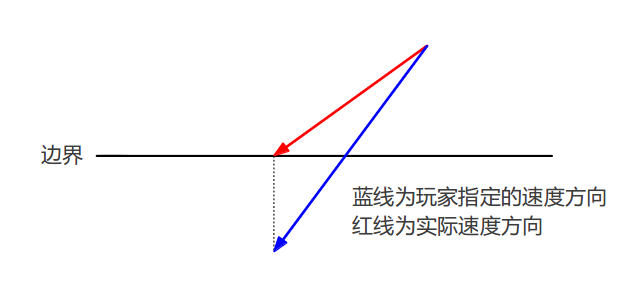
\includegraphics[width=0.5\textwidth]{side.png}
\caption{Plane移动出边界的修正}
\label{fig:side}
\end{figure}
\end{enumerate}

\end{document}
